%%%%%%%%%%%%%%%%%%%%%%%%%%%%%% -*- Mode: Latex -*- %%%%%%%%%%%%%%%%%%%%%%%%%%%%
%% project.01.29.tex -- 
%% Author          : Philip Johnson
%% Created On      : Tue Nov  4 10:26:48 1997
%% Last Modified By: 
%% Last Modified On: Mon Jan 29 09:03:18 2007
%% RCS: $Id$
%%%%%%%%%%%%%%%%%%%%%%%%%%%%%%%%%%%%%%%%%%%%%%%%%%%%%%%%%%%%%%%%%%%%%%%%%%%%%%%
%%   Copyright (C) 1997 Philip Johnson
%%%%%%%%%%%%%%%%%%%%%%%%%%%%%%%%%%%%%%%%%%%%%%%%%%%%%%%%%%%%%%%%%%%%%%%%%%%%%%%
%% 

\section{Introduction}

The goal of the Science of Design (SoD) program is to bring creative,
scientific advances to the design of software artifacts and systems.  New
paradigms, concepts, approaches, models, and theories arising from this
program should improve the processes of constructing, evaluating, and
modifying software-intensive systems. Important research questions include
the design and evaluation of software architectures with respect to their
quality and understandability; design optimization in the presence of
contradictory, inconsistent, emergent, and/or ambiguous requirements; and
analysis of tradeoffs between information and software design.  In all
cases the program focus is on basic research to advance the science of
software-intensive design, and on the effective application of SoD research
outcomes to the design of practical software intensive systems and their
integration into educational curricula.

The programmatic emphasis on ``creative'' approaches implies a preference
for revolutionary over evolutionary advances, and interdisciplinary over
single discipline approaches.  The programmatic emphasis on ``scientific''
approaches implies that the creativity should be framed within a
methodological context that supports, for example: (1) The ability to
characterize the internal and external validity of the findings; (2) The
ability to replicate the results; (3) Operational definitions for design
characteristics and outcomes relevant to the research, such as ``quality'',
``complexity'', ``performance'', ``usability'', ``maintainability'', and so
forth; and (4) Systematic measurement of qualitative and quantitative
metrics.

One impact of the Science of Design program results from the potential for
each project to discover one or more new design techniques with advantages
over the current state of the art in certain contexts of use.  This ``first
order'' impact could be augmented if at least some of these independent
findings are generated in a way that supports direct comparison,
combination, and/or meta-analysis with other findings.  This
facilitates  research on ``second-order'' impacts, such as
``Does the combination of new design technique X with new design technique
Y have an additive, multiplicative, or negative effect on software
quality?''  Comparability also accelerates the process of discovering the
context variables associated with research results, such as the types of
software or organizational contexts that support (or preclude) the use of a
new design technique.

A common way to facilitate direct comparison, combination, and meta-analysis is
through the use of a testbed.  One approach to testbeds is a common
artifact on which multiple design techniques can be applied and the results
compared.  For example, in the High Dependability Computing Project
\cite{Boehm04}, the SCRover software was developed as a common artifact for
assessing different dependability techniques \cite{Boehm04b}. A second
approach to testbeds is an experimental infrastructure for standardized
definition, collection, and analysis of empirical measures. For example,
the LDRA Testbed uses both static and dynamic instrumentation for process
improvement, testing, and maintenance \cite{Hennel06}.  Both kinds of
testbeds are useful, and indeed complementary: you could use an
infrastructure testbed to instrument the result of applying design
techniques to a common artifact.

To facilitate both first and second order impacts, the Science of
Design solicitation requests a special category of proposals focused on
``Demonstration Testbeds''.  These testbeds should support the development
of research infrastructures that enable evaluation of the utility and
quality of the artifacts produced by the Science of Design research
community.

In this project, we propose to design and implement a new testbed called
``SoDeT'' (Science of Design evaluation Testbed), which will be based
upon the Hackystat Framework \cite{Hackystat}.  The open source Hackystat
Framework has been under development in our lab for five years and has been
used in a wide variety of research and industrial settings. To use 
Hackystat, one attaches ``sensors'' to tools in order to capture
both ``process'' and ``product'' data about the software under development.

By process data, we typically mean developer behaviors that can be detected
through their interaction with a tool.  For example, by instrumenting an
interactive development environment, Hackystat can detect developer
behaviors such as when code is compiled, unit tests are invoked, and so
forth.  Because Hackystat attaches timestamps to these events, it can
provide a record of the sequence of behaviors that occur.

By product data, we mean information produced by the invocation of analysis
tools on a software artifact.  This can include size or structural
complexity metrics; the count and types of quality assurance problems
detected by tools like Checkstyle, PMD, FindBugs; source evolution over
time as captured by the configuration management system; and so
forth. While most of our experience with Hackystat involves the automated
collection of quantitative data, we have also investigated manual
collection of qualitative data, such as developer engineering logs.

SoDeT will leverage existing Hackystat support for over 30 sensors for a
wide variety of programming languages and tool frameworks. Because of this,
the SoDeT testbed will be able to instrument not only the new
design-specific tools and techniques developed as part of an SoD project,
but also other tools and processes employed in conjunction with the design
innovation.  For example, one SoD project focusses on a novel approach to
software testing and its interaction with design.  By instrumenting not
only to specific test tool developed by the SoD project, but also other
elements of the development environment, it becomes easier to investigate
``contextual'' questions, such as whether the SoD technique works within an
agile process such as Test Driven Design.

The SoDeT project is designed according to the following five objectives:

{\em 1. Provide a useful, usable demonstration testbed to a significant
number of Science of Design projects.} To achieve this objective, we have
already undertaken a preliminary feasibility study, the results of which are presented in
Section \ref{sec:preliminary-study}, and which we will build upon during the
project by a detailed feasibility study, as discussed in Section
\ref{sec:detailed-study}.

{\em 2. Improve the scientific benefits and research impact of individual
Science of Design projects.} The testbed will achieve this objective by
facilitating standard ways to define and collect outcome measures of interest to SoD
researchers, such as design ``quality'', ``reliability'', and ``cost''.
This improves the internal validity of the research, and facilitates replication
of SoD experiments in new contexts. 

{\em 3. Decrease the cost of empirical data collection and analysis for
design-oriented software research.}  By producing a useful, usable testbed
for Science of Design projects, a broader impact will be the creation of an
open source empirical infrastructure that should be helpful beyond the SoD
community to any design-oriented research efforts involving empirical
evaluation.

{\em 4. Facilitate comparative and/or meta analysis of individual
projects.} As noted above, the impact of the Science of Design program will
be amplified if individual research projects generate results in a form
amenable to comparison, combination, or statistical analysis with at least
some of the other projects.  The SoDeT testbed, by providing standardized
definition and collection mechanisms, can facilitate the integration of
individual results.

{\em 5. Facilitate discovery of high impact ``second order'' research 
opportunities.}  Also as noted above, an important future research direction
is to assess the opportunities that result from combining individual 
research advances.  The SoDeT testbed is designed to  both help in the 
discovery of potentially useful combinations, as well as provide a framework
that can facilitate understanding and assessment of the outcome of combining
various techniques together. 

The next section of this proposal presents a study of current SoD projects
that was undertaken in order to assess the feasibility of SoDeT.  The
following section presents related work, including the Hackystat Framework
and its relationship to other forms of testbeds.  We next present our plan
for how we intend to facilitate voluntary adoption of the SoDeT Testbed by
SoD participants. We conclude with a discussion of how this proposal
fulfills the NSF Merit Review criteria.

\section{A preliminary feasibility study}
\label{sec:preliminary-study}

\begin{figure*}[t]
\small
\begin{tabular}{|p{0.70in}|p{1.85in}|p{1.85in}|p{1.85in}|} \hline
{\bf PI(s)/ \newline (Response)} & {\bf Project Focus} & {\bf Tools Produced} & {\bf Outcome Measures/Hypotheses} \\ \hline

Abdelwahed (+)&
Model-based real-time, \newline  embedded system design &
Model-based design, analysis, \newline verification tools  &
(Improved) design, \newline (Improved) implementation \\ \hline

Amoussou &
Design Education &
None indicated &
None indicated  \\ \hline

Bailey &
Early stage UI design &
Visual sketching language, Early stage creative design tool &
None indicated  \\ \hline


Basili, \newline Carver &
Architectural change management &
None indicated  &
Models of architectural change, faults, design \\ \hline

Batory &
Generative Programming &
None indicated &
(Improved) program synthesis, optimization, and evolution \\ \hline

Bodik (+)&
Programming by sketching &
Sketching Synthesizer for Scientific Programs &
None indicated \\ \hline

Boehm (+)&
Value-based design &
Value-based software design tools &
None indicated \\ \hline

Bultan &
Design for Verification &
None indicated &
None indicated \\ \hline

Devanbu &
Open source design &
None indicated &
None indicated  \\ \hline

Ernst (-)&
Software design and testing &
Test generation from designs &
(Improved) execution, \newline (Improved) coverage \\ \hline

Findler \newline Felleisen &
Software markets, quality assurance, and design &
None indicated &
None indicated \\ \hline

\end{tabular} 
\caption{Feasibility of SoD projects for SoDeT adoption (Part 1 of 4)}
\label{fig:sod-1}
\normalsize
\end{figure*}

\begin{figure*}[ht]
\small
\begin{tabular}{|p{0.70in}|p{1.85in}|p{1.85in}|p{1.85in}|} \hline
{\bf PI(s)/ \newline (Response)} & {\bf Project Focus} & {\bf Tools Produced} & {\bf Outcome Measures/Hypotheses} \\ \hline

Fischer &
Participative software design &
Meta-design framework &
(Improved) participation \\ \hline

Flanagan &
Ethics and politics in design &
Values-in-design toolkit &
None indicated \\ \hline

Flatt, \newline Shivers &
Language ``towers'' &
Meta-tools for language design &
(More efficient) language design \\ \hline

Gamboa &
Design comprehensibility &
Enhanced Daikon, \newline Enhanced AbsInt &
Design quality (comprehensibility) \\ \hline

Getoor &
Semantic data integration, transformation, and sharing &
Data viewers, mappers, transformation languages &
None indicated \\ \hline

Goel &
Teleological Reasoning in Design &
Interactive software design environment &
Efficacy of teleological-based design  \\ \hline

Guzdial &
End-user programming &
None indicated &
None indicated \\ \hline

Hicks (+)&
Software Design Evaluation &
Tools for software design evaluation &
None indicated \\ \hline

Jackson \newline Perry (+)&
``Prescriptive'' software architecture descriptions &
Alloy constraint system \newline Compositional Compiler  &
(Improved) design quality \newline (Improved) design trade-offs \\ \hline

Jagadish (-)&
Incremental design of XML information systems &
Automated mapping/translation of schema &
(Reduced) effort to design and maintain information stores \\ \hline

Klein &
Non-linear negotiation for design &
Taxonomic knowledge base of designs &
(Improved) component choice, \newline (Improved) design efficiency \\ \hline

\end{tabular} 
\caption{Feasibility of SoD projects for SoDeT adoption (Part 2 of 4)}
\label{fig:sod-2}
\normalsize
\end{figure*}

\begin{figure*}[ht]
\small
\begin{tabular}{|p{0.70in}|p{1.85in}|p{1.85in}|p{1.85in}|} \hline
{\bf PI(s)/ \newline (Response)} & {\bf Project Focus} & {\bf Tools Produced} & {\bf Outcome Measures/ \newline Hypotheses} \\ \hline

Liu \newline Stoller &
Reconciling modularity and efficiency &
Language for design knowledge &
Design invariants \\ \hline

Lorenz \newline Attie &
Design locality &
``Pairwise composition'' analysis and verification tools &
Modular, modifiable, and maintainable designs \\ \hline

Mok \newline Abdelzaher &
Embedded software design &
Feedback control and stability tools &
(Improved) reliability \newline (Reduced) cost \\ \hline

Paul &
Multiprocessor chip design &
None indicated. &
None indicated \\ \hline

Rajlich &
Design of incremental change &
Static program analysis &
(Improved) quality \newline (Reduced) maintenance costs \\ \hline


Reiss &
Semantic component design &
None indicated &
(More controllable) design \\ \hline

Robinson (+)&
Requirements Monitoring, \newline End-user goals &
Run-time compliance monitor &
None indicated \\ \hline

Roth (+)&
Learning based programming &
Hybrid imperative/machine-learning language &
(Better) programming abstractions \\ \hline


Shaw &
Managing uncertainty in design &
None indicated &
(Reduced) user uncertainty \\ \hline

Sheard &
Semantics-based system design &
Omega &
None indicated  \\ \hline

Shipman &
Design by end-user &
End-user design tool \newline Design Repository &
(Improved) stakeholder communication, involvement \\ \hline


\end{tabular} 
\caption{Feasibility of SoD Projects for SoDeT adoption (Part 3 of 4)}
\label{fig:sod-3}
\normalsize
\end{figure*}

\begin{figure*}[ht]
\small
\begin{tabular}{|p{0.75in}|p{1.85in}|p{1.85in}|p{1.85in}|} \hline
{\bf PI(s)/ \newline (Response)} & {\bf Project Focus} & {\bf Tools Produced} & {\bf Outcome Measures/ \newline Hypotheses} \\ \hline

Sreenivas &
Design of discrete event system supervisory policies &
None indicated &
(Improved) discrete event system designs \\ \hline

Siskind (-)&
Functional programming &
None indicated &
None indicated \\ \hline

Su &
Business Process Specification &
Business Process Design, \newline Business Process Management &
(Reduced) development time, \newline (Improved) code quality \\ \hline

Sullivan \newline Griswold  (+)&
Economic analysis of design &
None indicated &
Economic ``value'' of designs \\ \hline

Taha &
Synthesizing device drivers &
MetaOCaml &
(Improved) design process \\ \hline

Tanimoto (+)&
Collaborative Design &
Communication,  evaluation tools, T-Star &
None indicated \\ \hline

Taylor (-) &
Architectural Design &
Tools for applying ``proven'' architectural styles &
None indicated \\ \hline


Vardi &
Automated design &
Assertion based automated design tool &
(Higher) quality, \newline (Shorter) design cycles \\ \hline

Xie &
Feedback-based architectures &
Tools for mission-critical software &
(Improved) reliability, \newline (Reduced) cost \\ \hline

Zhou &
Design and specification with imperfect components &
Model-based analyzer, verifier &
Functional limits of feasible systems \\ \hline

\end{tabular} 
\caption{Feasibility of SoD projects for SoDeT Adoption (part 4 of 4)}
\label{fig:sod-4}
\normalsize
\end{figure*}

Given that there are at least two fundamentally different approaches to
testbeds (artifact and infrastructure), and a wide variety of different
projects being pursued in the Science of Design program, a basic question
for any testbed is: ``If you build it, will they come?''  In other words,
given that it is unlikely (and probably undesirable) for a single SoD
testbed to be mandated for use by all SoD projects, what is the likelihood
that a significant number of SoD projects will voluntarily adopt an SoD
testbed for use in their research?

Based upon our experience with external adoption of Hackystat over the past
several years, we believe that the answer to this question will depend upon two
properties of the SoDeT testbed: utility and usability.  The utility of a testbed
concerns the degree to which it provides support for answering the research
questions of interest to the project leaders.  In the case of SoDeT, the
utility question for an SoD project leader translates to, ``Can the SoDeT
testbed gather process and product metrics that helps me answer interesting
questions about my design innovation?''

Even if the SoDeT testbed has potential utility to an SoD project, it will not be
adopted unless it has an adequate level of usability.  Usability refers to
the level of effort required to install, configure, and use the testbed.
In the case of SoDeT, the usability question for an SoD project leader
translates to, ``How much time will be required from me or my staff to
install the SoDeT testbed, configure it for use in my project, gather the data,
and interpret the results?''

To provide some initial insight into the utility question with respect to
the SoDeT testbed, we searched the NSF Awards database for all currently
funded Science of Design awards. After eliminating awards for workshops and
consolidating multiple awards for team-based projects, we were left with 43
distinct projects. For these 43 projects, we reviewed the project abstract
to see if we could extract the following information: (1) An indication of
what kinds of design tools would be produced from the project, if any; (2)
What kinds of ``outcomes'' would be produced by the project, and (3)
whether the project abstract contained reference to any testable, empirical
hypotheses, such as ``improved'' quality or ``decreased'' cost.

Since the Awards database results included the PI name and contact email,
we also sent an email to each PI to gather more direct information about
the project.  In our email, we briefly introduced the SoDeT testbed
approach and asked two questions: (1) if their research would produce a
tool that appeared to be amenable to our form of testbed instrumentation,
and (2) would their research produce an empirical measure of one or more
design or implementation characteristics, such as ``quality'',
``goodness'', ``faults'', ``efficiency'', and so forth.

Figures \ref{fig:sod-1}, \ref{fig:sod-2}, \ref{fig:sod-3}, and
\ref{fig:sod-4} contain a summary of the results of our award abstract
review and email request to the PIs. (The projects are listed in
alphabetical order by PI name. The results are split into four tables
purely for page layout purposes.)  The first column contains the name(s) of
the PI(s).  It also contains a ``(+)'' if a PI replied to our email with a
generally positive response concerning our two questions, and a ``(-)'' if
a PI replied with a generally negative response.  We received responses
to our email regarding 13 out of the 43 projects (30\%).

The second column presents a phrase summarizing the focus of the project
based upon our review of the abstract.  The third column lists the tools
produced by the project, or ``None indicated'' if the abstract did not
indicate that tools would be produced.  The fourth column lists measurable
outcomes mentionned in the abstract if the research is successful.  If the
abstract indicates a testable hypothesis, the fourth column indicates that
using a parenthesized comparator, such as ``(Improved)'', ``(Reduced)'',
``(Higher)'', ``(Shorter)'', and so forth.

Before beginning the interpretation of this data, it is important to
understand the limitations of this preliminary feasibility study.
First, it is not possible to gain deep insight into a project from a one
paragraph description.  This means that we may have misconstrued the
presence/absence of tools or outcomes for certain projects.  In the same
way, since our email contained only a one paragraph description of the
SoDeT testbed approach, it is possible that the responding PIs may have
been inappropriately positive (or negative) concerning its applicability to
their research.  Nevertheless, while we accept that there is considerable
uncertainty with respect to the correctness of our analysis of any
individual project, we hope that the aggregate analyses will provide at
least coarse evidence regarding the degree of compatibility between the
SoDeT testbed approach and the Science of Design program as a whole.

To begin, one capability of the SoDeT testbed is tool instrumentation,
which can simplify collection of data such as when a tool is invoked, the
outcome of the tool's invocation, the amount of time spent executing the
tool, and so forth.  If an SoD project does not produce a tool, then it is
less likely that this kind of data will be of interest.  From our analysis,
30 of the 43 project abstracts (70\%) indicate that a tool would be
produced as part of the research.  Thus, a substantial number of projects
at least qualify for tool instrumentation, though it remains unclear as to
whether SoDeT tool data would provide the project leaders with useful
insight regarding their research questions.

A second capability of SoDeT is to provide standard, operational
definitions for measures and a consistent framework with which to collect
and analyze them.  For example, five of the project abstracts include the
same testable hypothesis: that their tools and techniques will result in
``improved design quality''.  Of course, there are many different
definitions for ``quality'', many different types of artifacts that could
be considered a ``design'', and many different levels of ``improvement''.
The goal of the SoDeT framework is {\em not} to coerce different projects
to agree to use the same measures.  Instead, the goal is for the framework
to be both sufficiently flexible and powerful so that project leaders can
define and collect the measures of interest to them more easily than they
could by ``handrolling'' their own measurement infrastructure.  If that is
accomplished, then use of the framework results a more precise
understanding of the differences between the measures designed by each
project, and creates opportunities for meaningful meta-analysis.  From our
analysis, 19 of the 43 project abstracts (44\%) included a potentially
testable hypothesis, and 26 out of 43 project abstracts (60\%) included
either a potentially testable hypothesis or an empirical outcome measure.

In summary, looking at the tool column alone indicates 70\% of the projects
are potentially appropriate, and looking at the Outcome Measures/Hypotheses
column alone indicates that 60\% of the projects are potentially
appropriate.  If this analysis approach is appropriate, then we would
predict that projects designed to produce both a tool and outcome
measure/hypothesis would be the most likely to be amenable to the SoDeT
testbed, and we would likewise predict that projects producing neither a
tool nor an outcome measure/hypothesis would be least likely to be
interested.  The tables reveal that 20 out of 43 project abstracts (47\%)
mention both a tool and an outcome measure/hypothesis, 16 out of 43 project
abstracts (37\%) mention either a tool or an outcome measure/hypothesis,
and the remaining 7 project abstracts (16\%) mention neither a tool nor an
outcome measure/hypothesis.

The email responses from PIs are generally consistent with these
percentages: 9 out of 13 replies (69\%) indicated a potential interest in
applying the SoDeT testbed approach to their project.  Unfortunately, the
project abstract analysis results and the email results are not entirely
consistent.  For example, two of the four negative email responses came
from projects whose abstracts indicate that they will produce both a tool
and an outcome measure/hypothesis.  The third negative email had no outcome
measure/hypothesis indicated in their abstract, and the fourth negative
email had neither a tool nor an outcome measure/hypothesis.

The preceding feasibility analysis addresses only the ``utility'' question;
it does not provide insight into the ``usability'' of SoDeT.  Some
indirect insight into SoDeT usability can be inferred from usability
research on the Hackystat Framework \cite{csdl2-03-12,csdl2-07-02}.  The
first study revealed problems with client-side installation of sensors,
which was addressed through a client-side GUI installer wizard.  The latest
usability study of Hackystat has initiated a redesign of its server-side
web application user interface to incorporate Ajax and other ``Web 2.0''
features.  Despite these issues, Hackystat is currently usable enough for
application in a variety of academic and industrial contexts, as discussed
in Section \ref{sec:hackystat}.

In conclusion, this preliminary feasibility analysis appears to indicate
that the testbed approach embodied by SoDeT will be feasible from a utility
point of view to approximately half of the current SoD projects.  If we
assume that, in a similar way, approximately half of those projects find
SoDeT to be adequately usable, then a conservative estimate for the number
of SoD projects using the SoDeT testbed is 6 to 12.  A more optimistic estimate,
starting with the email reply percentages as a basis, is approximately double
the conservative estimate, or 12 to 24 projects.

\section{Related Work}

\subsection{Hackystat}
\label{sec:hackystat}


For the past five years, we have been developing a framework for
automated software development process and product metric collection and
analysis called Hackystat.  This framework differs from other approaches to
software product and process measurement in one or more of the following ways:

\begin{itemize}

\item Hackystat uses sensors to unobtrusively collect data from development
environment tools; there is no chronic overhead on developers to collect
product and process data.  In contrast, tools such as the Process Dashboard
\cite{PSPDashboard} involve manual data collection. 

\item Hackystat is tool, environment, process, and application agnostic.
The architecture does not suppose a specific operating system platform, a
specific integrated development environment, a specific software process,
or specific application area.  A Hackystat system is configured from a set
of modules that determine what tools are supported, what data is collected,
and what analyses are run on this data. In contrast, tools such as TSP Tool
\cite{TSPTool} implement support for a fixed set of metrics under a fixed
process on a single platform.

\item Hackystat is intended to provide in-process project management
support. Traditional software metrics approaches, such as 
the NASA Metrics Data Program \cite{MDPRepository},  are based upon the
``project repository" method, in which data from prior completed projects
are used to make predictions about a future
project. In contrast, Hackystat is designed to continuously collect data from a current,
ongoing project, and use that data as feedback into the current project.

\item Hackystat is open source and is available to the academic and
commercial software development community for no charge. In contrast,
commercial toolkits such as MetricCenter \cite{MetricCenter} are closed
source and require licensing fees.

\end{itemize}

The design of Hackystat \cite{csdl2-02-07} reflects prior 
research in our lab on software measurement, beginning with research into
data quality problems with the PSP \cite{csdl-98-11} and continuing with
research on the LEAP system for lightweight, empirical, anti-measurement
dysfunction, and portable software measurement \cite{csdl2-00-03}.

\begin{figure*}[ht]
  \centering
  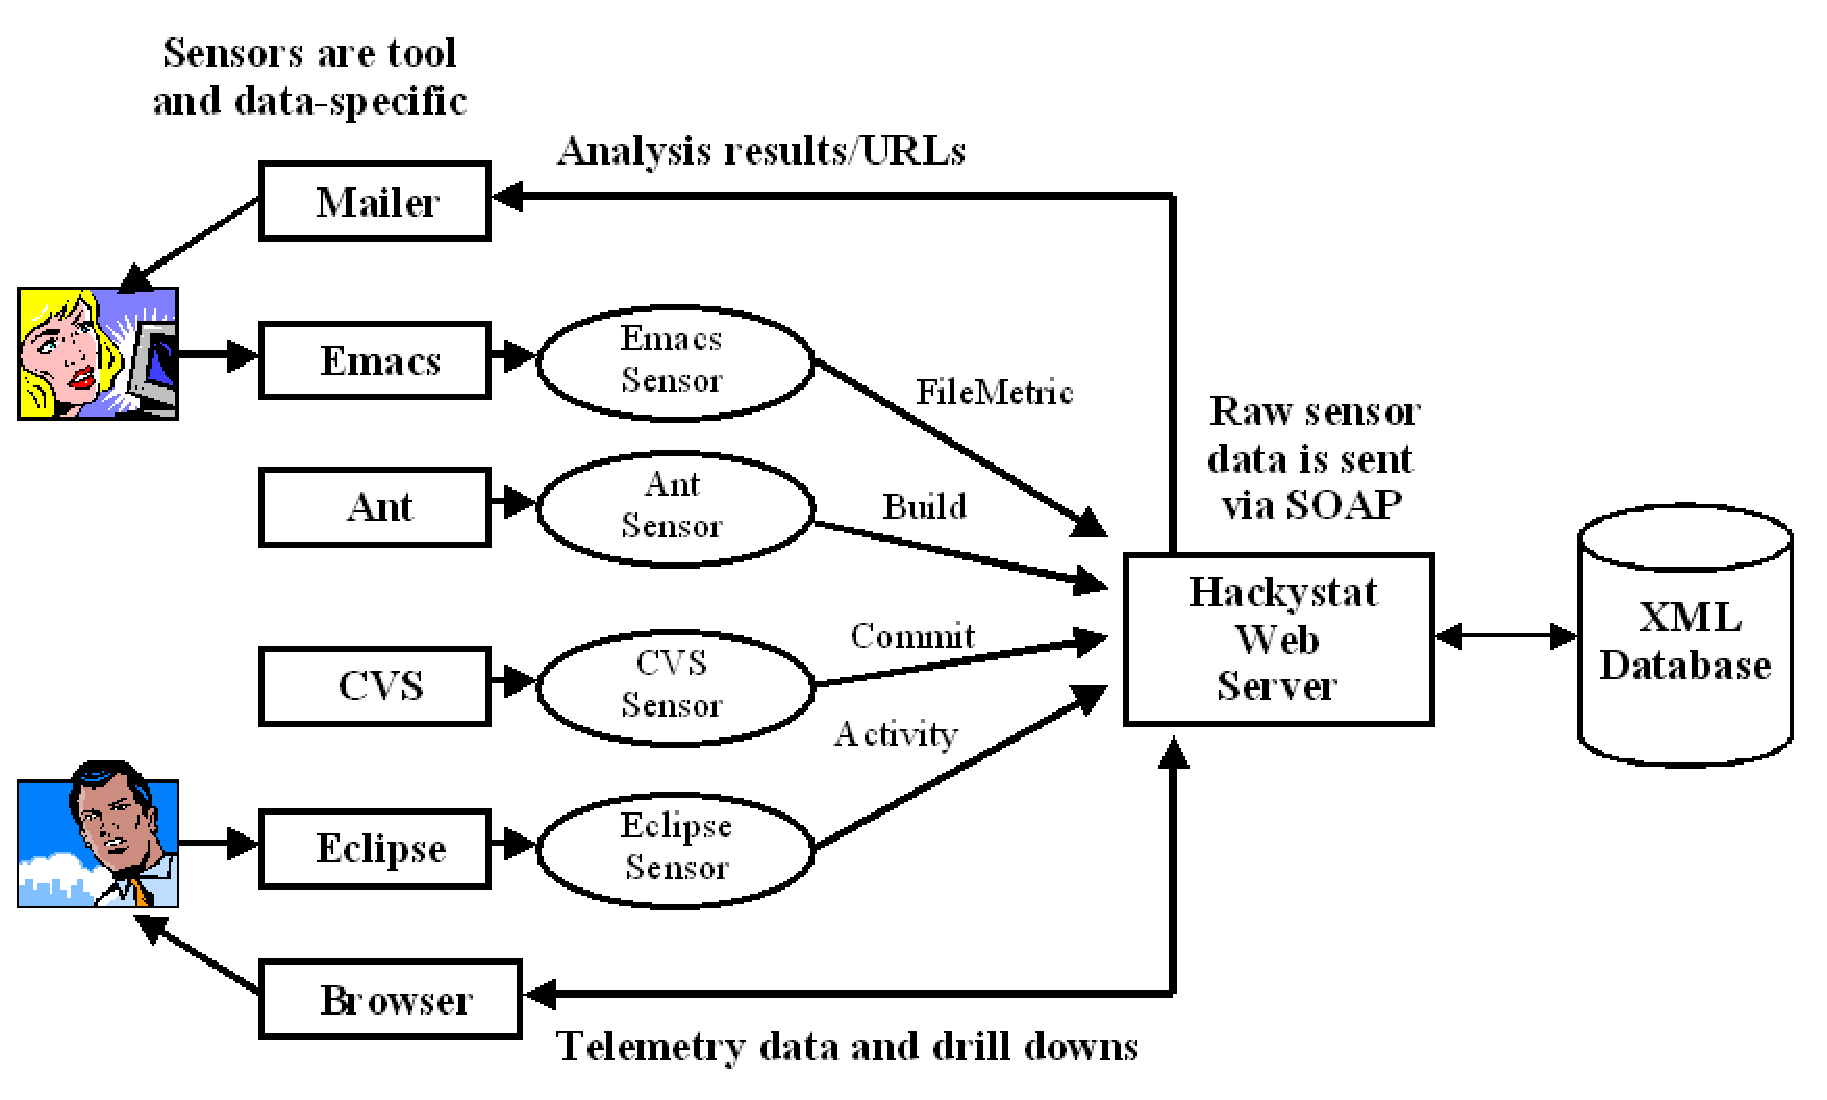
\includegraphics[width=0.60\textwidth]{architecture.eps}
  \caption{The basic architecture of Hackystat.}
  \label{fig:architecture}
\end{figure*}

To use Hackystat, the project development environment is instrumented by
installing Hackystat sensors, which developers attach to the various tools
such as their editor, build system, configuration management system, and so
forth. Once installed, the Hackystat sensors unobtrusively monitor
development activities and send process and product data to a centralized
web server.  If a user is working offline, sensor data is written to a
local log file to be sent when connectivity can be re-established.  Project
members can log in to the web server to see the collected raw data and run
analyses that integrate and abstract the raw sensor data streams into
telemetry.  Hackystat also allows project members to configure ``alerts``
that watch for specific conditions in the sensor data stream and send email
when these conditions occur. Figure \ref{fig:architecture} illustrates the
basic architecture of the system.

Hackystat is an open source project. Its sources, binaries, and
documentation are freely available online.  We also maintain a public
server running the latest release of the system at
http://hackystat.ics.hawaii.edu.  Hackystat has been under active
development for approximately five years, and currently consists of
approximately 2500 classes and 300,000 lines of code.  Sensors are available
for a variety of tools including Eclipse, Emacs, JBuilder, Jupiter, Jira,
Visual Studio, Ant, JUnit, JBlanket, CCCC, DependencyFinder, Harvest, LOCC,
Office, CVS, and SVN.

Hackystat is being used in a variety of academic and industrial contexts.
At the University of Hawaii, Hackystat has been  integrated into the
undergraduate and graduate software engineering curriculum, and is
used by approximately 50 students per year to support project
development \cite{csdl2-03-12}.  A researcher from the Free University of
Bozen came to Hawaii to study the Hackystat system in support their research on
PROM \cite{Sillitti03}.  Researchers at the University of Maryland are
using Hackystat to support assessment of programmer effort
\cite{Hochstein05}.  Hackystat has been used at NASA's Jet Propulsion
Lab to analyze the daily build process for the Mission Data System
\cite{csdl2-03-07}.  Finally, Hackystat is being used at SUN Microsystems
to support research on high performance computing system development
productivity \cite{csdl2-04-03}.

In fact, one of
its current applications is as a testbed for evaluation of the design
technique known as Test Driven Design (TDD) \cite{csdl2-06-02}.

\subsection{Comparative and Meta Analysis}

We believe that no single study gives unequivocal results.
Therefore, it is imperative that the research community try 
to integrate and compare
studies that address a common hypothesis. This is the only way to gain 
confidence that empirical results are real and not just due to random 
variation. However, integrating multiple studies in a credible way isn't
simple. In this case, the two studies address the same issue, but they were 
conceived and executed independently. Thus, direct comparison of the results
is impossible because the studies differ considerably in their designs, 
instrumentation, subject population, and analysis methods.
 
A classic approach to understanding what several studies say about 
some phenomenon is to conduct a literature review, qualitatively 
summarize existing results, and manually synthesize them. The drawback 
of this approach is that it lacks precise methods for combining 
different results. 

A statistical approach for integrating multiple studies is called 
meta-analysis. This approach has two steps. First, the 
experimenters attempt to reconcile the primary experiments -- i.e define 
a common framework with which to compare different studies.  This involves
defining common terms, hypotheses, and metrics, and characterizing key 
differences.  Next, the data from the primary experiments are transformed 
or recalculated according to agreed upon definitions. In the second step
the transformed primary data is combined and reanalyzed.
Unfortunately, it is not always clear when meta-analysis is appropriate,  
what statistical models should be used, or when it is acceptable to 
combine data from disparate sources. 

A recent revolution in medical research involves the introduction of an
``evidence-based'' paradigm.  This paradigm arose in response to two
observations: the failure to organize medical research into systematic
reviews could cost lives, and the clinical judgement of experts compared
unfavorably with the results of systematic reviews.   The evidence-based 
approach is starting to be applied outside of medicine, in fields such as
psychiatry, nursing, social policy, education, and software engineering. 

Kitchenham has been leading the movement for evidence-based software
engineering, organizing workshops on this topic and publishing papers
explaining the issues involved in applying evidence-based research
techniques to software engineering \cite{Kitchenham04,Kitchenham04a}.  She
and her collaborators propose a five step method for evidence-based
software engineering: (1) Convert the need for information [about a
software engineering practice] into an answerable question; (2) Track down
the best evidence available for answering the question; (3) Critically
appraise that evidence using systematic review for its validity (closeness
to the truth), impact (size of the effect), and applicability (usefulness
in software development practice); (4) Integrate the critical appraisal
with current software engineering knowledge and stakeholder values [to
support decision-making]; (5) Evaluate the effectiveness and efficiency in
applying Steps 1-4 and seek ways to improve them for next time.  While
promising, application of systematic reviews and the integration of
empirical software engineering data from multiple sources has been found to
be challenging \cite{Jedlitschka04}.

\subsection{Results from prior NSF research}

\begin{tabular}{lp{4.5in}}

Award number: & CCF02-34568 \\
Program: & Highly Dependable Computing and Communication Systems Research\\
Amount: & \$638,000 \\
Period of support: & September 2002 to September 2007 \\
Title of Project: & Supporting development of highly dependable software through
continuous, automated, in-process, and individualized software measurement validation \\
Principal Investigator: & Philip M. Johnson \\
Selected Publications: & \cite{csdl2-04-22,csdl2-04-13,csdl2-04-11,csdl2-03-12,
csdl2-02-07,csdl2-03-07,csdl2-04-02,csdl2-04-04,csdl2-04-06}
\end{tabular} \\ %[3mm]


\section{Project Plan}

The SoDeT testbed project is organized into six phases: 
(1) Detailed feasibility analysis, (2) Testbed kickoff, (3) Testbed
implementation and enhancement, (4) Trial adoption, (5) Testbed
deployment, and (6) Testbed wrapup.  The following sections describe
the goals and activities of each phase.  

\subsection{Detailed feasibility analysis}
\label{sec:detailed-study}

One useful outcome of the preliminary feasibility analysis presented 
earlier in this proposal is that determining the utility and usability
of a given testbed for a given SoD project is difficult without detailed
knowledge of both the testbed and the project.  Our conclusions from the
project abstracts were based upon detailed knowledge of the testbed but
superficial knowledge of the project; conversely, the conclusions in the
email responses were based upon detailed knowledge of the project but
superficial knowledge of the testbed. 

The first stage of this project is therefore to perform a more
detailed feasibility analysis.  To do this, we will contact the
current SoD award PIs, introduce the SoDeT testbed project, and explain
that we are conducting a feasibility analysis of the testbed. We
will then request that they provide us with a copy of the 15 page ``Project
Description'' section of their Science of Design proposal as well as any
other related research artifacts they believe would be helpful in our 
effort.

Based upon this more detailed project description and any other related
artifacts, we will perform an analysis with three outcomes.

The first outcome will be a detailed, individual feasibility analysis of
the SoDeT testbed for each SoD project.  This feasibility analysis will be
provided back to the PI(s) of the corresponding project for review and
feedback.  This analysis will consider at least the following issues: (1)
what specific forms of process or product data could be collected by the
testbed that would appear to be useful to the project; (2) what specific
kinds of analyses could be performed upon this data that would appear to
provide relevant findings for the research project; (3) what kinds of
methodological impact the use of the testbed would have on the project,
such as changes to the experimental evaluation method; (4) a recommendation
from our perspective as to whether the SoDeT testbed appears to be worth
pursuing by the project; and (5) if worth pursuing, what would be the
appropriate initial step by the project leaders to evaluate for themselves
the utility and usefulness of SoDeT.  Through iteration with the PIs, we
will refine this analysis until it represents a consensus viewpoint on the 
feasibility of the testbed for each project. 

The second outcome will be a set of new requirements for the SoDeT testbed
which will be needed in order to maximize its utility and usability to the
SoD community.  We expect these requirements to include: (1) new types of
sensors for the tools developed by the community or used as part of their
research process; (2) new kinds of sensor data types to represent the novel
forms of design issues and representations produced by the project,
including qualitative data representations; (3) new forms of analyses which
might or might not build upon existing Hackystat applications such as
Software Project Telemetry or SDSA; and (4) new forms of interface to
support appropriate communication of the analyses to the researchers and/or
designers.

The third outcome will be a document proposing a set of new projects with
``second order'' Science of Design research impact.  The new projects will
focus on possible ways in which the SoDeT testbed could facilitate new
kinds of research that integrates together existing independent SoD
projects.  An example of a loosely coupled form of integration would be to
collect the same type of sensor data in the same way by the different
sensors attached to the design tools produced by different projects.
Subsequent processing by a common analysis would reveal similarities and
differences between the application of the two design tools, at least with
respect to this form of data.  It may also reveal interesting insights into
the differences between the two contexts of application of the two tools.

An example of a more tightly coupled form of integration would be a project
in which two or more instrumented design tools or techniques are available
for application within the same development context.  A variety of
interesting research questions can be posed within this environment. For
example, if the use of all the tools is mandated, what is the impact on
outcome measures such as quality or efficiency?  How is usage of the
various design tools interleaved?  What is the impact of these tools on the
usage of other tools?  If the use of all the tools is not mandated, which
tools are voluntarily employed, when are they used, and what are the
outcomes of their usage?  

\subsection{Testbed kickoff}

Once the detailed feasibility analysis is completed, the SoDeT testbed will
be formally introduced to the community at a ``Kickoff'' presentation.  If
the timing for the Kickoff coincides with the yearly SoD PI meeting, we
will request time to do it there, otherwise we will conduct an online
web-based presentation (``webinar'') using commercial tools available for
that purpose such as WebEx or GoToWebinar.  At that meeting, we will
present the results of the detailed feasibility analysis stage to the
entire community for review and feedback.  For those projects that have
agreed to take the next step in evaluating SoDeT for use, we will provide
information on what steps should be taken next. 

While we will present and solicit feedback on the ``second order'' research
impact projects, we do not expect any formal commitment to these projects
at such an early date in the testbed research process. Instead, the goal at
this point is to catalyze a dialogue within the community on what kinds of
second order impacts are desirable and feasible, and how to move toward
that kind of research over time.

\subsection{Testbed implementation and enhancement}

As soon as SoDeT requirements become available, we will begin implementing 
the enhancements required to the Hackystat framework to support the SoD
projects for which a consensus on feasibility was reached.  As the SoDeT 
testbed will leverage the Hackystat Framework, it is possible in best case
scenarios that only simple sensor and analysis enhancements will be required,
and for those projects a SoDeT testbed configuration could be available within 
a few weeks.  

We expect that we will receive a steady stream of enhancement requests from the
SoD community over the course of the project, and that the implementation and
enhancement activities will be substantial and ongoing throughout the course of 
the project. 

\subsection{Trial adoption}

As a first step toward SoDeT usage, an SoD project will download and
install a configuration of the SoDeT testbed loaded with the sensors,
analyses, and user interface features appropriate to their research as
revealed during the detailed feasibility analysis.

This configuration will then be applied to a pilot study by the SoD project
members.  The goals of the pilot study are to enable the SoD project members to 
become familiar with the use of the testbed to collect and analysis data, and 
to help discover any additional requirements for use not found during the 
detailed feasibility analysis stage.  

\subsection{Testbed deployment}

If the trial adoption stage is completed successfully, the SoD project can
move into full deployment of the testbed to collect the process and product
data in a scientifically useful manner. For example, while the pilot study
phase might use members of the SoD project team itself for data collection,
this phase might use the testbed to collect data from students randomly
assigned to treatment groups, or from industrial users.

We anticipate that even during testbed deployment, the SoD projects will
uncover additional requirements and desirable enhancements to the SoDeT
testbed, which we will do our best to implement and distribute in a timely
manner.

\subsection{Testbed wrapup}

In the final six months of the project, we will transition out of
development and support mode and into a ``wrapup'' phase with two primary
activities.

The first activity is the development of an ``Experience Base''
\cite{Basili94} that provides insights into the lessons we learned about the
development of a Science of Design testbed and its deployment in the
research program.  The goal is to provide transferable knowledge to other
NSF programs in which testbed infrastructure is desired, so that our
experience can be replicated with greater efficiency and impact.  The open
source SoDeT testbed will also be available as a reference to support this
tech transfer activity.

The second activity during this wrapup phase of the project is collaborative
with the SoD PIs to refine and improve the initially proposed set of
``second order'' research projects in light of the data and outcomes of the
individual projects.  The goal of this activity is to generate an agenda
for a new round of SoD research in which comparison, replication, and
meta-analysis are explicit goals of the program.

\subsection{Work breakdown structure}

Figure \ref{fig:wbs} provides a work breakdown structure that shows when
each of these phases begins and ends during the project and how they
overlap in time.  We split each year into two six month periods: ``Fall'' 
lasts from July to December, and ``Spring'' lasts from January until June.

\begin{figure*}[ht]
  \centering
  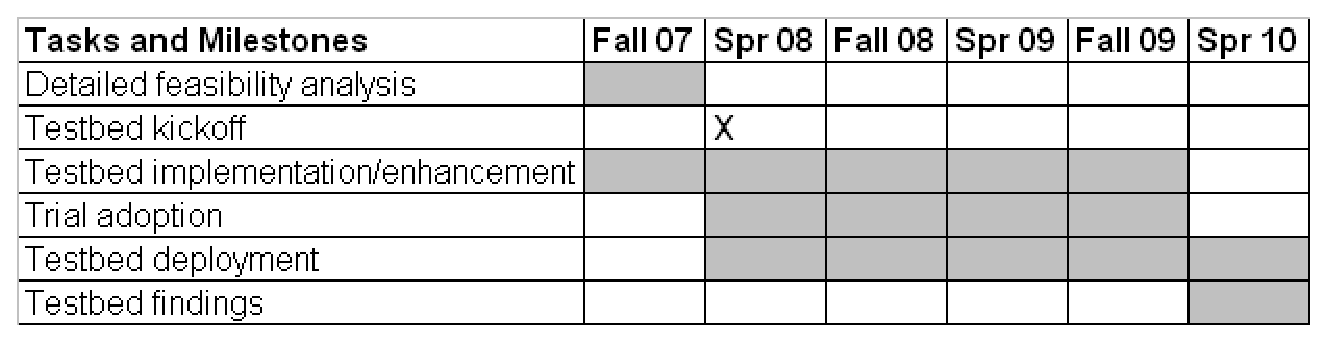
\includegraphics[width=0.75\textwidth]{workstructure.eps}
  \caption{Work breakdown structure and milestones.} 
  \label{fig:wbs}
\end{figure*}

Assuming that this project begins in Fall, 2007, we anticipate finishing the Detailed feasibility
analysis phase within six months.  This enables the Testbed kickoff meeting to occur in early 
Spring, 2008.  

Testbed implementation and enhancement will begin as soon as information begins to be available
as a result of the Detailed feasibility analysis, and will continue throughout the project until 
the last six months, at which point the focus will shift to ``wrapup'' activities. 

Trial adoption by participating SoD research groups should start in Spring 2008 and is expected
to continue for the next year or two.  We anticipate that for any individual research project,
the trial adoption phase will last a few weeks to a few months, but that research projects will
become ready to undergo Trial adoption at varying times over the course of this project.

Similarly, the Testbed deployment phase could start as soon as Spring 2008 for some SoD
projects, but could start as late as Spring 2010 for others.  The duration of the deployment 
phase for any given SoD research project is purely a function of their project and its goals. 
In some cases, the Testbed might be used for only a few weeks to conduct a controlled experiment, 
while others might use it for a longitudinal case study lasting many months. 

Finally, the Testbed wrapup phase will occupy the final six months of the project. 

\section{Conclusions}
\label{sec:merit}

NSF Science of Design proposals are evaluated according to their
intellectual merit, broader impacts, and new, creative ways to think about
a Science of Design discipline.

The SoDeT testbed has the potential to significantly advance knowledge and
understanding within the Science of Design program.  It can accomplish this
in several ways. First, it can provide new, standardized, comparable ways
to operationalize the empirical measurement of design characteristics
produced by individual SoD projects.  This can both raise the quality of
research results from individual projects, and enable forms of
meta-analysis across multiple projects that might not have been possible
without a common framework for process and product data collection and
analysis.

Second, the SoDeT testbed can significantly reduce the cost to individual
researchers of data collection and analysis. Use of the testbed reduces the
need by individual projects to develop custom data collection software, or
to alternatively employ manual data collection techniques, which are more
time-consuming, less scalable, and error-prone.

Third, this year's solicitation expresses the desire to ``look forward in
the near future to the effective application of SoD research outcomes to
the design of practical software-intensive systems''.  The SoDeT testbed is
designed to provide instrumentation support for laboratory, classroom, and
industrial environments.  It can thus facilitate more rapid technology
transfer of the design innovations from laboratory to ``real-world''
environments, providing high quality data back to the researchers that can
help them to recognize and respond to issues as they arise in new settings.

Fourth, our feasibility analysis indicates that a significant number of SoD
projects are designed in such a way as to potentially benefit from the SoDeT 
testbed.  

The broader impacts of this research project result from the fact that the
SoDeT testbed, being based on the Hackystat Framework, can be easily
applied outside the context of the Science of Design program. As an open
source project, the SoDeT testbed will be freely available for use and
adaptation.  

The SoDeT Testbed can also improve educational opportunities in software
design.  The Hackystat Framework is used regularly in educational settings
to teach about software engineering measurement, and the SoDeT testbed
enhancements can be adapted to this environment to support teaching about
new design innovations and their impact upon design characteristics.

As the University of Hawaii is a university with 75\% minority students in
an EPSCOR state, a final broader impact of this project is the potential
for it to provide novel research opportunities to underrepresented groups.

